\documentclass[tikz,dvisvgm,border=0pt]{standalone}
% Shared preamble of the diagrams in vignettes/articles/cuda-kernels.Rmd.
% Render them with `make diagrams` from the package root.
\usepackage[T1]{fontenc}
\usepackage{lmodern}
\usepackage{tikz}
\usetikzlibrary{arrows.meta, positioning, fit, backgrounds, calc, shapes.geometric, decorations.pathreplacing}

\definecolor{host}{HTML}{3B6EA8}
\definecolor{device}{HTML}{2E8B57}
\definecolor{accent}{HTML}{C0571B}
\definecolor{muted}{HTML}{6B6B6B}

% A white card behind every figure, so that it reads in pkgdown's dark mode.
\tikzset{
  every picture/.append style={
    show background rectangle,
    background rectangle/.style={fill=white, rounded corners=6pt},
    inner frame sep=8pt,
    font=\sffamily\small,
    >={Stealth[length=2.2mm]},
  },
  box/.style={draw, rounded corners=3pt, thick, align=center, inner sep=5pt, fill=white},
  hostbox/.style={box, draw=host, fill=host!8},
  devbox/.style={box, draw=device, fill=device!8},
  accbox/.style={box, draw=accent, fill=accent!8},
  region/.style={draw=#1, rounded corners=6pt, thick, dashed, inner sep=8pt},
  heading/.style={font=\sffamily\bfseries\small, text=#1},
  note/.style={font=\sffamily\footnotesize, text=muted, align=center},
  flow/.style={->, thick},
  code/.style={font=\ttfamily\footnotesize},
}

\begin{document}
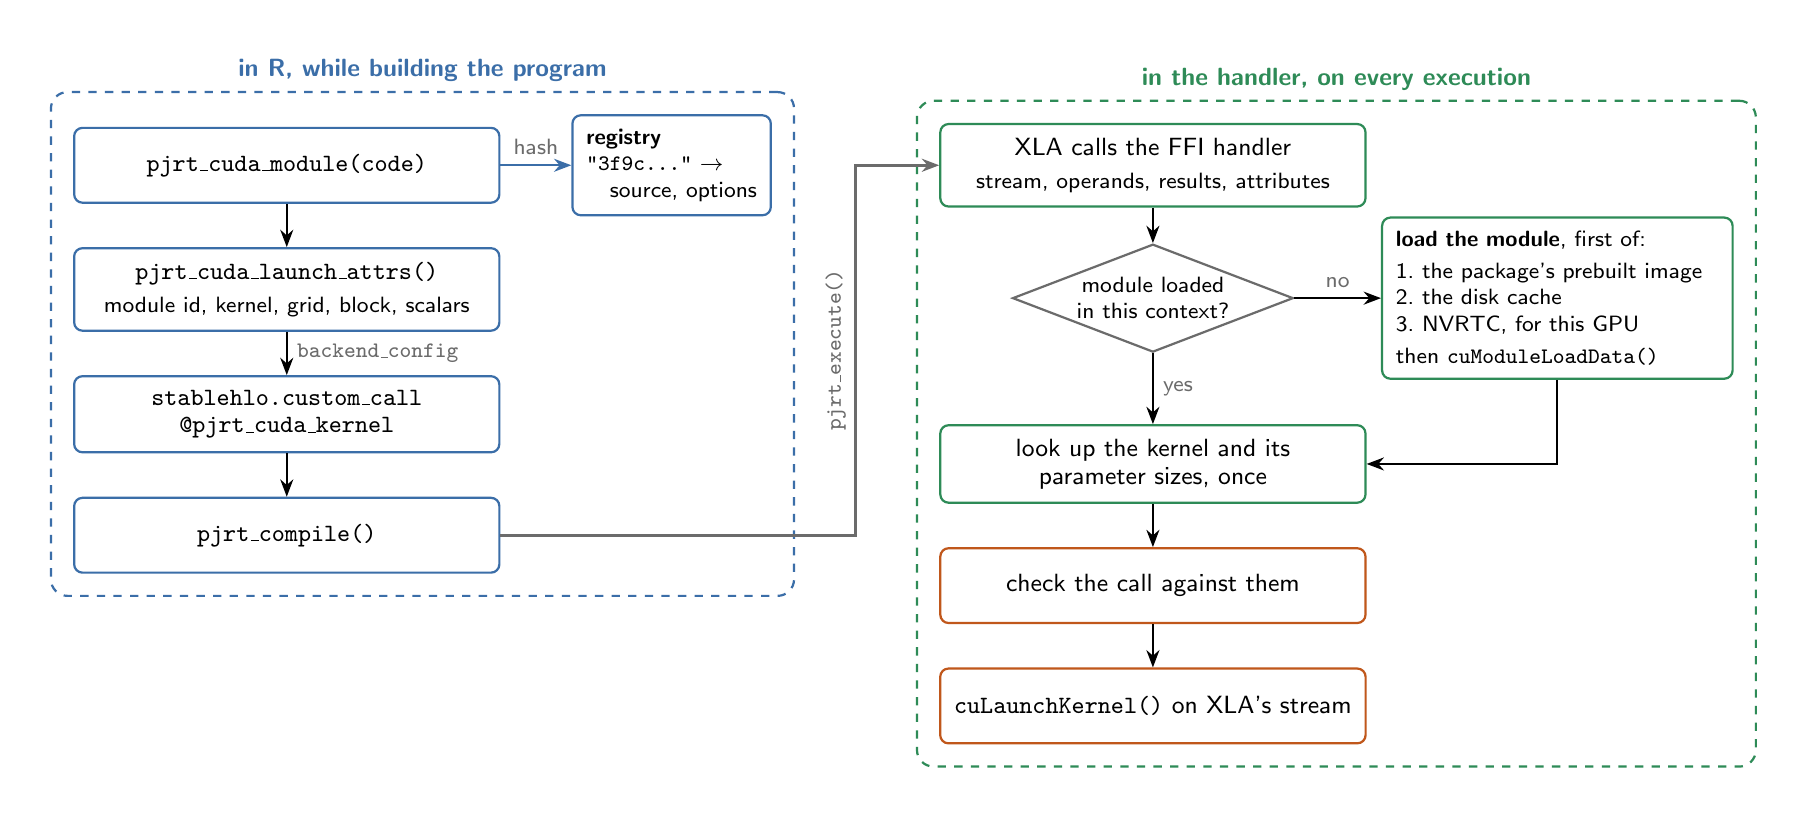
\begin{tikzpicture}[
    stage/.style={box, minimum width=5.4cm, minimum height=0.95cm},
    q/.style={diamond, aspect=2.6, draw=muted, thick, fill=white, inner sep=1pt, align=center, font=\sffamily\footnotesize},
  ]
  % ---- in R, once
  \node[hostbox, stage] (mod) at (0, 0) {\texttt{pjrt\_cuda\_module(code)}};
  \node[hostbox, stage, below=0.55cm of mod] (attrs) {\texttt{pjrt\_cuda\_launch\_attrs()}\\[1pt]{\footnotesize module id, kernel, grid, block, scalars}};
  \node[hostbox, stage, below=0.55cm of attrs] (hlo) {\texttt{stablehlo.custom\_call}\\[-1pt]\texttt{@pjrt\_cuda\_kernel}};
  \node[hostbox, stage, below=0.55cm of hlo] (comp) {\texttt{pjrt\_compile()}};
  \draw[flow] (mod) -- (attrs);
  \draw[flow] (attrs) -- node[right, note] {\texttt{backend\_config}} (hlo);
  \draw[flow] (hlo) -- (comp);
  \node[box, draw=host, right=0.9cm of mod, font=\sffamily\footnotesize, align=left] (reg)
    {\textbf{registry}\\\texttt{"3f9c\ldots"} $\to$\\\quad source, options};
  \draw[flow, host] (mod) -- node[above, note] {hash} (reg);
  \node[region=host, fit=(mod)(comp)(reg), label={[heading=host]above:in R, while building the program}] (rside) {};

  % ---- in the handler, every execution
  \node[devbox, stage] (call) at (11.0, 0) {XLA calls the FFI handler\\[1pt]{\footnotesize stream, operands, results, attributes}};
  \node[q, below=0.45cm of call] (loaded) {module loaded\\in this context?};
  \node[devbox, stage, below=0.9cm of loaded] (fn) {look up the kernel and its\\[-1pt]parameter sizes, once};
  \node[accbox, stage, below=0.55cm of fn] (check) {check the call against them};
  \node[accbox, stage, below=0.55cm of check] (launch) {\texttt{cuLaunchKernel()} on XLA's stream};
  \draw[flow] (call) -- (loaded);
  \draw[flow] (loaded) -- node[right, note] {yes} (fn);
  \draw[flow] (fn) -- (check);
  \draw[flow] (check) -- (launch);

  % the load chain
  \node[box, draw=device, anchor=north west, text width=4.1cm, align=left, font=\sffamily\footnotesize, right=1.1cm of loaded.east, anchor=west] (chain)
    {\textbf{load the module}, first of:\\[2pt]
     1.\ the package's prebuilt image\\
     2.\ the disk cache\\
     3.\ NVRTC, for this GPU\\[2pt]
     then \texttt{cuModuleLoadData()}};
  \draw[flow] (loaded.east) -- node[above, note] {no} (chain.west);
  \draw[flow] (chain.south) |- (fn.east);
  \node[region=device, fit=(call)(launch)(chain), label={[heading=device]above:in the handler, on every execution}] (cside) {};

  \coordinate (gap) at ($(rside.east)!0.5!(cside.west)$);
  \draw[flow, very thick, muted] (comp.east) -- (comp.east -| gap) |- (call.west);
  \node[note, rotate=90, anchor=south] at ($(gap |- comp.east)!0.5!(gap |- call.west)$) {\texttt{pjrt\_execute()}};
\end{tikzpicture}
\end{document}
